% !TeX root = ../main.tex
% Add the above to each chapter to make compiling the PDF easier in some editors.

\chapter{\glsentrytext{holoassistapp}s}\label{chapter:holoassistapps}

As previously stated, one of the main aims of this project is to enable researchers with limited computer science experience to create and test \gls{AR} experiences inside a flight simulator. One of the reasons for which \gls{holoassist} has been designed as a standalone application that exposes an high-level \gls{API} was precisely this: asking someone with limited programming background to become familiar with C\#, Unity, the Mixed Reality Toolkit and the workflow required to develop on the Hololens was simply not feasible. Using \gls{holoassist}'s \gls{API} over the local network is significantly easier, but it can be simplified further.

To do this, it was decided to create a \enquote{paved road}\cite{marsh_paved_nodate} that could act as a starting point and preferred way to use \gls{holoassist}'s \gls{API}. The Python programming language\cite{noauthor_python_nodate} was the obvious choice for the foundation of this paved road: its pseudo-code-like syntax, dynamically typed nature and runtime safety make it (comparatively) easy to use, also for inexperienced programmers. The trade-off is that Python is a really slow interpreted language, even when compared with similar languages. Fortunately, this disadvantage is overcome by the immense collection of open-source libraries and packages that are available online\cite{noauthor_pypi_nodate}: some of them, like Numpy\cite{noauthor_numpy_nodate} or Scypi\cite{noauthor_scipy_nodate}, offer easy to use Python bindings to extremely performant scientific computation libraries written in low-level languages like C, C++ or Rust. Installing these packages and using them is almost trivial (especially if compared to the alternatives) and this allows to deal with Python's performance problems. Combining this with the availability of other packages that cover a large number of scientific computing necessities (e.g.\ PyProJ\cite{noauthor_pyproj_nodate} for geodesy, Skyfield\cite{rhodes_skyfield_nodate} for astronomy, Matplotlib bindings\cite{noauthor_matplotlib_nodate} for plotting, PyTorch\cite{noauthor_pytorch_nodate} for deep learning, and many more) makes for a very strong value proposition, which has lead to an ever increasing adoption of the Python language and ecosystem (see \autoref{fig:stack_overflow_developer_survey.png}). This makes it therefore more likely for aspiring users of \gls{holoassist} to already be familiar with this language.

\begin{figure}
  \centering
  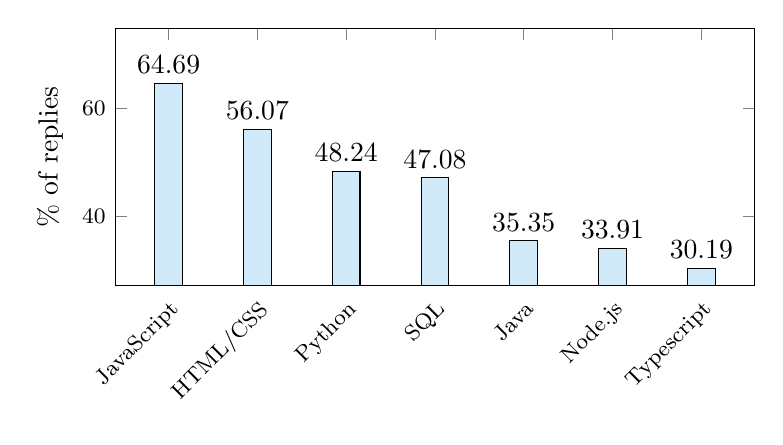
\begin{tikzpicture}
    \definecolor{myblue}{RGB}{13,98,153}
    \definecolor{mybluefill}{RGB}{208,234,250}

    \begin{axis}[
        symbolic x coords={JavaScript, HTML/CSS, Python, SQL, Java, Node.js, Typescript},
        xtick=data,
        width=0.8\textwidth,
        height=0.4\textwidth,
        x tick label style={rotate=45, font=\footnotesize, anchor=north east}, 
        y tick label style={font=\footnotesize}, 
        ylabel = {\% of replies},
        nodes near coords,
        ymin=27, ymax=75
    ]
        \addplot[ybar,black,fill=mybluefill] coordinates {
            (JavaScript, 64.69)
            (HTML/CSS, 56.07)
            (Python, 48.24)
            (SQL, 47.08)
            (Java, 35.35)
            (Node.js, 33.91)
            (Typescript, 30.19)
        };
    \end{axis}
\end{tikzpicture}

  \caption{The 2021 Stackoverflow Developer Survey\cite{noauthor_stack_nodate} reports Python as the third most-popular language among developers, up one position with respect to the previous year. The plot shows the results of the question \enquote{Which programming, scripting, and markup languages have you done extensive development work in over the past year?}}\label{fig:stack_overflow_developer_survey.png}
\end{figure}

After deciding the language for the paved road, the next step was to create a Python class (\texttt{HoloAssistService}) that would act as a wrapper for \gls{holoassist}'s \gls{API}: in this way, users only have to invoke normal Python methods on instances of this class and not have to worry about the details of the network protocol and the format chosen for data serialization. After creating this class, the only remaining steps were to write the appropriate documentation and to create a few example \glspl{holoassistapp} that would use this paved road and could act as a starting point for others that will be developed in the future.

\section{Example \glsentrytext{holoassistapp}s}\label{sec:example_holoassistapps}

The simplest \gls{holoassistapp} that could be developed is one that highlights a particular landing strip of an airport, and is reported in its entirety in \autoref{lst:highlight_eddm_api_code}. Obtaining the geographical coordinates of the corners of the landing strip can be done through Google Maps. Once these coordinates are known, the \gls{holoassist} \gls{API} can be used to create the rectangular line mesh that will highlight the desired runway. Doing this requires building a list containing the vertices of the rectangle and a list that defines the lines connecting these vertices. This second list is known as the list of indices, because its elements are the numerical indices of the vertices defined in the first list. Each pair of elements of the list of indices describes a line with endpoints the two vertices identified by the corresponding indices. This approach is similar to how triangular meshes are commonly represented in 3D computer graphics, and its details are explained in \autoref{sec:geofixedaug_representation}. Meshes created through the \gls{holoassist} \gls{API} in this way are known as \gls{gfelm} in this document. In order to send the list of vertices and the list of indices to \gls{holoassist}, the \texttt{HoloAssistService} class offered by the paved road can be used. It offers a wrapper around the raw \gls{API} which allows to invoke it by simply calling normal Python methods. The result created by this \gls{holoassistapp} is shown in \autoref{fig:eddm_highlighted.png}.

\begin{figure}
  \centering
  \begin{tabular}{c}
  \begin{lstlisting}[language=python]
    from lib import prepare_holo_assist_instance
    from lib.holo_assist_types import Color, GeoFixedVertex, WGS84Point

    c = Color(0.0, 1.0, 0.0) #RGB
    vertices = [
      GeoFixedVertex(WGS84Point.from_degrees(48.3630, 11.7675, 453), c),
      GeoFixedVertex(WGS84Point.from_degrees(48.3671, 11.8210, 453), c),
      GeoFixedVertex(WGS84Point.from_degrees(48.3666, 11.8212, 453), c),
      GeoFixedVertex(WGS84Point.from_degrees(48.3625, 11.7676, 453), c)
    ]

    indices = [0, 1, 1, 2, 2, 3, 3, 0]
    MESH_ID = "EDDM 08 L"

    service = prepare_holo_assist_instance()
    service.create_mesh(MESH_ID)
    service.add_mesh_vertices(MESH_ID, vertices)
    service.add_mesh_indices(MESH_ID, indices)
    service.commit_mesh_changes(MESH_ID)
    service.activate_mesh(MESH_ID)
  \end{lstlisting}
  \end{tabular}
  \caption{An example \gls{holoassistapp} that highlights the \texttt{08 L} runway of the Munich airport (\texttt{EDDM}). The explanation of what each \gls{API} call does is available in \autoref{appendix:external_meshes_api}.}\label{lst:highlight_eddm_api_code}
\end{figure}

\begin{figure}
  \centering
  \includegraphics[width=0.8\textwidth]{eddm-runway-aligned.png}
  \caption{An image acquired from the Hololens that shows the visual result of one of the simplest \glspl{holoassistapp} that can be created.}\label{fig:eddm_highlighted.png}
\end{figure}

Another example \gls{holoassistapp} that was implemented shows how to take an arbitrary Wavefront OBJ line mesh and draw it at a specific geographical point. To achieve this result, a couple of utility methods to load such mesh file and to convert it to \texttt{GeoFixedVertices} have been developed and offered as part of the paved road. An example usage of these methods is shown in \autoref{lst:importing_an_obj_mesh}: the vertex and index lists it generates can then be used with the \gls{holoassist} \gls{API} as usual. The result that can be obtained from such \gls{holoassistapp} is shown in \autoref{fig:maps_pin_on_earth.png}. Creating a 3D mesh like this can be done in Blender, by drawing the desired shape, deleting all the faces (keeping therefore only vertices and edges) and by exporting the result as OBJ. As it can be seen in \autoref{lst:obj_to_geofixed_converter}, the mapping between the original mesh vertices and the \texttt{GeoFixedVertex} datastructure is straightforward and does not involve any computation, just a direct conversion.

\begin{figure}
  \centering
  \begin{tabular}{c}
  \begin{lstlisting}[language=python]
    COLOR = Color(0.0, 0.8, 0.0)
    POSITION = WGS84Point.from_degrees(48.36306, 11.76755, 453)
    ROTATION = Rotation.from_degrees(0, 0, 0)

    map_pin_obj = simple_obj_importer.load_obj_line_mesh("/path/to/mesh.obj")
    (vertices, indices) = convert_obj_to_geo_fixed_mesh(
      map_pin_obj, COLOR,
      POSITION, ROTATION
    )
  \end{lstlisting}
  \end{tabular}
  \caption{An example usage of the utility functions that convert a normal Wavefront OBJ line mesh to a format that can be sent as-is to \gls{holoassist}'s \gls{API}.}\label{lst:importing_an_obj_mesh}
\end{figure}

\begin{figure}
  \centering
  \begin{tabular}{c}
  \begin{lstlisting}[language=python]
    def convert_obj_to_geo_fixed_mesh(
      mesh: ObjLineMesh, mesh_color: Color,
      mesh_geo_position: WGS84Point,
      mesh_local_rotation: Rotation):

      vertices = [
        GeoFixedVertex(
          mesh_geo_position, mesh_color,
          Vector3(-point[0], point[1], point[2]),
          mesh_local_rotation
        ) for point in mesh.vertices
      ]

      flattened_indices = itertools.chain.from_iterable(mesh.lines)
      indices_in_base_zero = [i - 1 for i in flattened_indices]

      return (vertices, indices_in_base_zero)
  \end{lstlisting}
  \end{tabular}
  \caption{The paved road implementation of the conversion from Wavefront OBJ to \texttt{GeoFixedVertex}. It is fairly straightforward, although care should be taken to convert from Blender's right-handed coordinate system to Unity's (and HoloAssist's) left-handed coordinate system. That's the reason of the \enquote{-} sign applied to one of the coordinates of the mesh.}\label{lst:obj_to_geofixed_converter}
\end{figure}

\begin{figure}
  \centering
  \includegraphics[width=0.8\textwidth]{map-pin.png}
  \caption{An image acquired from the Hololens that shows how \glspl{holoassistapp} can be used to render arbitrary line meshes.}\label{fig:maps_pin_on_earth.png}
\end{figure}

The last example \gls{holoassistapp} focused on \glspl{geofixedaug} that has been developed is an adapter that is able to use \gls{holoassist}'s \gls{API} to draw a tunnel mesh starting from a CSV file written in a custom format in use at the research institute in which this project was developed. Luckily, each CSV line could be mapped one-to-one to an \gls{holoassist} \gls{API} call, therefore writing the adapter was fairly straightforward.

An example \gls{holoassistapp} that creates a \gls{planefixedaug} has also been created, obtaining the result shown in \autoref{fig:plane_fixed_aug_example.png}. 

\section{Augmenting the Innsbruck approach}

Besides the example \glspl{holoassistapp} described in \autoref{sec:example_holoassistapps}, the main test case for the developed platform was enhancing the landing experience for the Innsbruck airport. As the approach chart in \autoref{fig:lowi_approach_chart.png} shows, the airport is surrounded by mountains: this complicates the landing, especially in conditions of limited visibility. The main idea is that \gls{AR} could be used to highlight the elements relevant for the approach, improving the situational awareness of the pilot and leading to a safer landing.

\begin{figure}[p]
  \centering
  \includegraphics[width=0.8\textwidth]{lowi-approach.png}
  \caption{The approach chart to the Innsbruck airport for the procedure \texttt{RNP-Y-RWY-08}. This approach chart is offered for simulation use only by VACC-Austria\cite{vacc_austria_lowi_nodate}.}\label{fig:lowi_approach_chart.png}
\end{figure}

It was decided to focus on the standard procedure \texttt{RNP-Y-RWY-08}, shown in \autoref{fig:lowi_approach_chart.png}. This approach is for runway 08 which, due to the mountains surrounding the airport, requires performing a left turn shortly before actually landing. Especially with limited visibility conditions, following the correct trajectory can be fairly challenging. For such procedure, three elements were identified as relevant and useful to be highlighted:

\begin{enumerate}
    \item The airport landing strip;
    \item The mountains on the left side of the approach trajectory, as the aircraft needs to fly quite close to them to correctly follow the procedure;
    \item The desired approach trajectory itself, in the form of a tunnel inside which the airplane should stay.
\end{enumerate}

Each of these three elements was implemented independently in its own \gls{holoassistapp}.

The geographical coordinates of the runway corners were obtained via QGis, an open-source software designed for reading and writing \gls{GIS} data. The QGis project consisted of two layers: a base layer with the satellite imagery from Google Maps and a feature layer on which points and shape could be drawn. After drawing the runway outline on this layer, its content was exported to a GeoJSON\cite{butler_geojson_2016} file. The \texttt{geojson} Python package\cite{noauthor_geojson_nodate} was then used to read this file into an \gls{holoassistapp} that mapped its content to the datastructure required by \gls{holoassist}'s \gls{API}. The result is shown in \autoref{fig:innsbruck_runway_augmentation.png}.

\begin{figure}
  \centering
  \includegraphics[width=0.8\textwidth]{lowi-runway.png}
  \caption{The \gls{holoassistapp} that highlights the Innsbruck airport's runway.}\label{fig:innsbruck_runway_augmentation.png}
\end{figure}

Highlighting the mountains on the left side of the approach trajectory was less straightforward, as it required drawing a 3D mesh that would match their shape, at least roughly. Fortunately, the Austrian government (through its open data platform) has released a publicly available digital elevation model for the entire Austrian territory with a $10$m resolution, which is precise enough for this use case\cite{land_karnten_digitales_nodate}. In this model, each pixel represents a real world square with a side of $10$m and the color of the pixel encodes the average height of that real world square. The parameters of the mapping between the color and the real-world height are embedded in the the image metadata, as it is common for the GeoTIFF\cite{the_open_geospatial_consortium_ogc_2019} format in which it is distributed. Such metadata allows to effortlessly import it in the QGis project as another geo-referenced layer, which is then trimmed to the appropriate area of interest as shown in \autoref{fig:qgis_with_altitude.png}. This area, which surrounds the Innsbruck airport, is small enough for the Earth curvature to be negligible. This means that this chunk of the elevation model can be exported from QGis as a normal gray-scale image that can then be imported in Blender and be used as an height map to create virtual geometry that roughly matches the real world terrain. Such geometry can then be enhanced by exporting the Google Maps satellite view of that same area from QGis as a normal RGB image that can be then applied to the virtual geometry in Blender. This process results in an approximate digital reconstruction of the real-world that surrounds the Innsbruck airport. Such reconstruction is precise enough to be used as a starting point to draw a 3D mesh that could be used to highlight the mountains, as shown in \autoref{fig:mountains_wire_mesh.png}. This 3D mesh can then be exported to an OBJ file\footnote{Technical note. Before exporting from Blender, the mesh origin (that is, the Blender object position) must be moved back to $(0, 0, 0)^T$, otherwise the resulting augmentation will be misaligned} which can in turn be used by a \gls{holoassistapp} to be shown in the real simulator, as shown in \autoref{fig:lowi_full_terrain.png}.

\begin{figure}
  \centering
  \includegraphics[width=0.8\textwidth]{qgis-satellite-and-dem.png}
  \caption{The QGis project used for this \gls{holoassistapp}. It shows the satellite imagery of the Innsbruck airport area and the relevant part of the digital elevation model.}\label{fig:qgis_with_altitude.png}
\end{figure}

\begin{figure}
  \centering
  \includegraphics[width=0.8\textwidth]{3d-mountains-in-blender.png}
  \caption{A screenshot of the Blender project that was used to create the terrain 3D mesh for the area surrounding the Innsbruck airport. The mesh is highlighted in orange, whereas the rest of the 3D scenes is occupied by the digital reconstruction obtained by using the digital elevation model as a height map.}\label{fig:mountains_wire_mesh.png}
\end{figure}

\begin{figure}
  \centering
  \includegraphics[width=0.7\textwidth]{innsbruck-full-terrain.png}
  \caption{The final appearance of the highlighted terrain in the flight simulator.}\label{fig:lowi_full_terrain.png}
\end{figure}

During early testing, it was suggested that always showing the whole mountain mesh could easily become overwhelming. It was therefore decided to extend the terrain \gls{holoassistapp} so that only the part of the terrain mesh that is closer than a certain threshold is shown. The same simulator position data that updates \gls{holoassist} was therefore duplicated and made available also to the terrain \gls{holoassistapp}. While running, the app uses PyProj to convert all the \texttt{GeoFixedVertices} that compose the terrain mesh to their \gls{ECEF} position, using an algorithm similar to the one described in \autoref{eq:externallinemeshvertextoecef}. The current airplane position is also converted to the \gls{ECEF} \gls{CRS}, and the distance between each mesh point and the current airplane position is computed. If the distance is greater than the given threshold then the slots of the mesh's index list that refer to those vertices are set to zero (resulting in those mesh lines disappearing). If the distance goes back below the threshold then they are restored to their original value (making those mesh lines appear again). A few of the physical buttons of the simulator have been integrated (via their \gls{UDP} interface) in this \gls{holoassistapp} and allow the pilot to dynamically change the distance threshold at which vertices (and therefore parts of the terrain augmentation) are hidden. The fact that this is possible is a demonstration of the flexibility of the \gls{API} exposed by \gls{holoassist}, and the fact that the entire app only requires around $150$ lines of Python shows its ease of use and the maturity of the Python ecosystem for this kind of tasks.

The last \gls{holoassistapp} that has been developed for the Innsbruck airport shows a tunnel representing the correct approach trajectory that should be maintained by the aircraft to follow the given approach procedure. The approach procedure chosen for this example is \texttt{RNP-Y-RWY-08} (shown in \autoref{fig:lowi_approach_chart.png}), which is a required navigation performance procedure: this means that instead of describing the trajectory in terms of ground-based localization equipment, it uses a sequence of geographical points that the aircraft computer  follows\footnote{Of course, this is a simplified description of what a required navigation performace procedure is and only focuses on the aspects relevant for this project.}. This sequence of geographical points for \texttt{RNP-Y-RWY-08} has been obtained from the airport approach charts has been written in a CSV file which is then loaded by an \gls{holoassistapp}. Each of these points is treated as the center of a rectangle which forms a vertical cross-sectional slice of what will become the trajectory tunnel. The correct indices are then added to connect every corner of every cross-sectional slice to the respective corner of the previous and next cross-sectional slice, yielding the tunnel-like appearance shown in \autoref{fig:lowi_approach_only_linear_tunnel.png}.

\begin{figure}
  \centering
  \includegraphics[width=0.7\textwidth]{innsbruck-approach-linear.png}
  \caption{The visual result from of the first iteration of the \gls{holoassistapp} displaying the approach tunnel for the Innsbruck airport.}\label{fig:lowi_approach_only_linear_tunnel.png}
\end{figure}

Although this technique is simple to implement, it is not perfect, as the approach trajectory is just piece-wise linearly interpolated, leading to sudden changes of direction in proximity of the points defining the tunnel cross-sectional slices. On a real aircraft, its Flight Management System (FMS) would compute the ideal trajectory using the GPS data of the aircraft, its speed and its aerodynamic performance. However, due to the complexity of these algorithms, displaying the ideal approach trajectory was deemed to be beyond the scope of the current version of this \gls{holoassistapp}. Nevertheless, it was decided to try using a spline to smooth the piece-wise-linear interpolation.

To do this, the set of points loaded from the CSV file are transformed to the \gls{ECEF} Euclidean \gls{CRS} by using PyProj and are then interpolated with a cubic spline via Scipy. This spline is then evaluated at around $60$ different equally-spaced points, each of which is used as the center for rectangular cross-sectional slice of the approach tunnel. Such rectangle is oriented (by using the local rotation component of the \texttt{GeoFixedVertex} data structure) to be perpendicular to the ground and with its normal pointing towards the spline tangent at that point (and therefore \enquote{following} the spline). By connecting every rectangle with the previous and following one the result shown in \autoref{fig:lowi_spline_tunnel.png} is achieved.

\begin{figure}[b!]
  \centering
  \includegraphics[width=0.7\textwidth]{innsbruck-approach-spline.png}
  \caption{The visual result from of the second iteration of the \gls{holoassistapp} displaying the approach tunnel for the Innsbruck airport, using a tunnel based on a computed spline.}\label{fig:lowi_spline_tunnel.png}
\end{figure}

The combination of these three \glspl{holoassistapp} (shown in \autoref{fig:all_together_now}) leads to the result which will be shown to a few pilots to gather their feedback on this initial example of \gls{AR} techniques applied to an aircraft cockpit.

\begin{figure}[b!]
  \centering
  \includegraphics[width=0.7\textwidth]{all-together-now.png}
  \caption{The three \glspl{holoassistapp} developed for the Innsbruck airport.}\label{fig:all_together_now}
\end{figure}